\documentclass[aps,pre,superscriptaddress]{revtex4}

\usepackage{preamble}
\graphicspath{ {./figures} }

\begin{document}

% \begin{abstract}
% \end{abstract}

\title{SBM-WCC Ian's Document}
\author{Ian Chen}
\date{\today}
\maketitle

\section{Introduction}
See the preprint~\cite{Park25-02}.

\section{Materials and Methods}

\section{Nested-SBM on Empirical Networks}

\begin{figure}
	\centering
	\begin{subfloat}
		\centering
		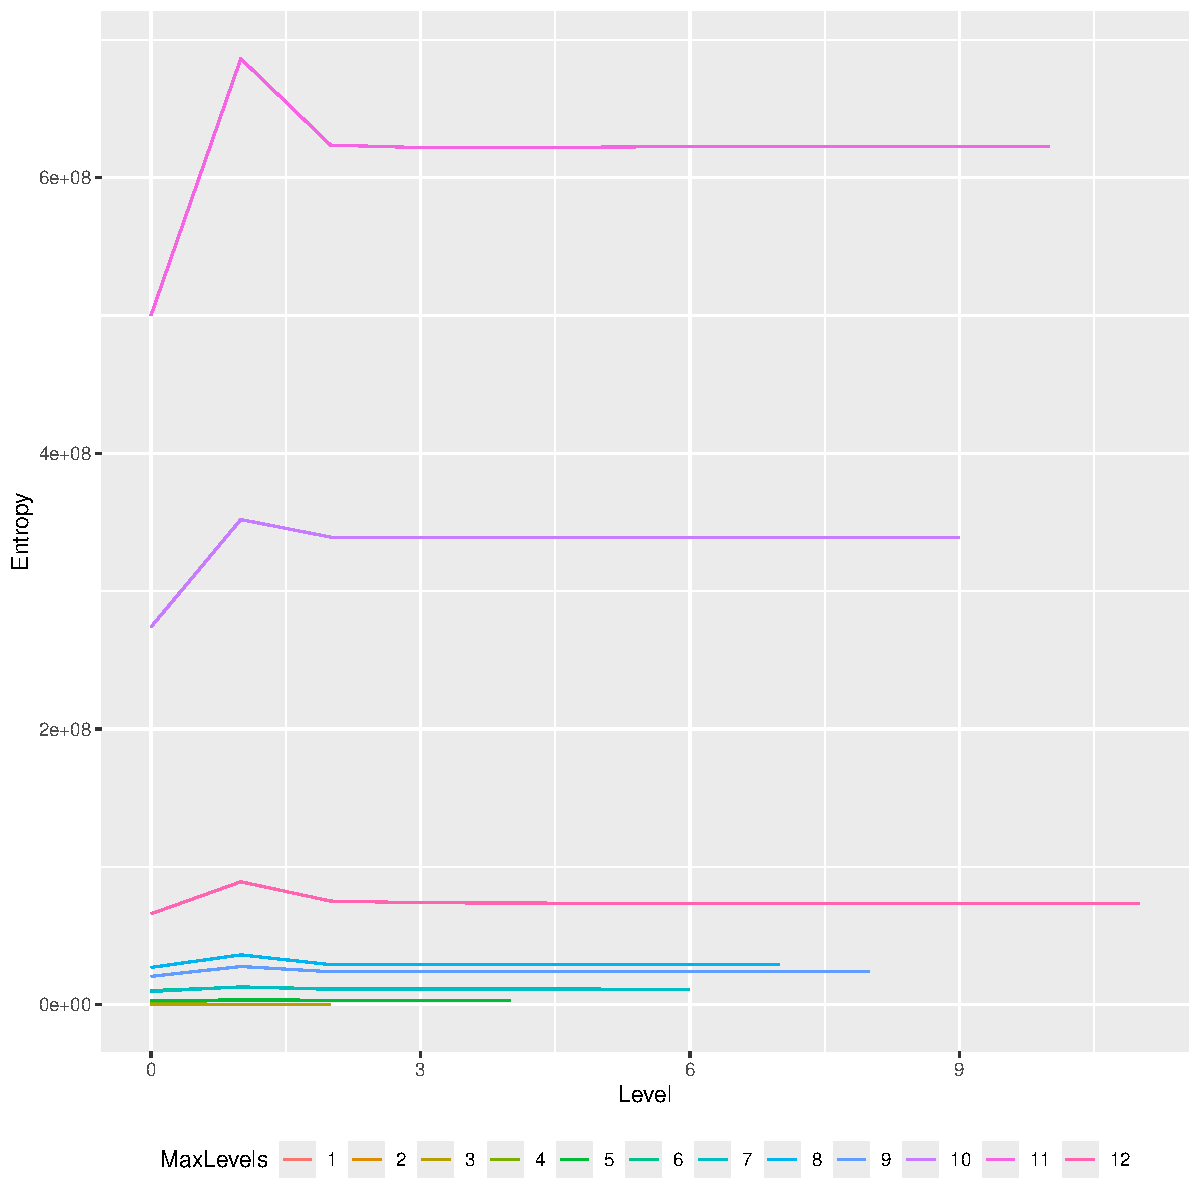
\includegraphics[width=0.48\textwidth]{fig1.pdf}
	\end{subfloat}
	\begin{subfloat}
		\centering
		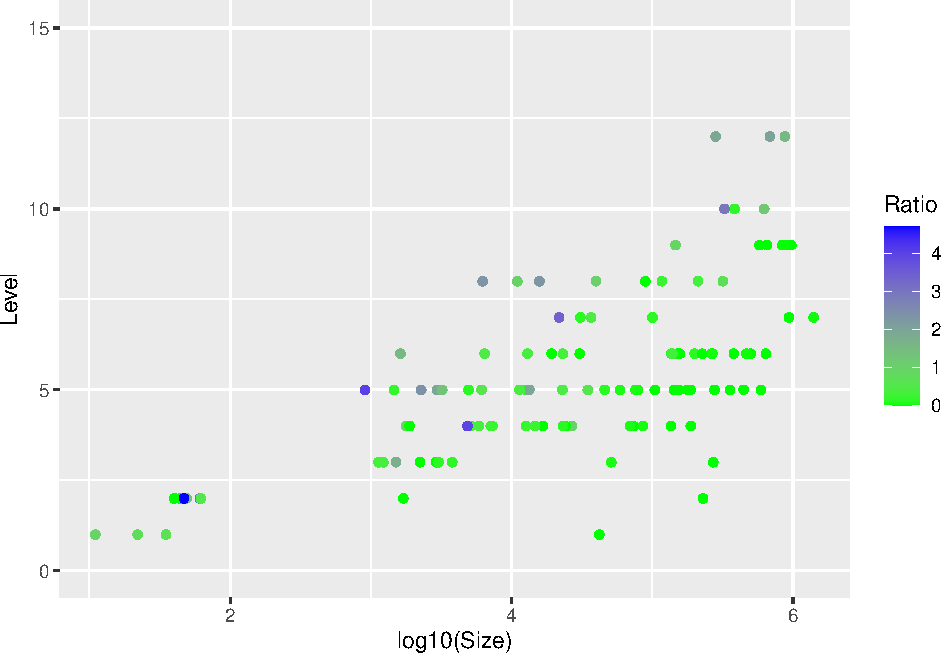
\includegraphics[width=0.48\textwidth]{fig2.pdf}
	\end{subfloat}
	\caption{Entropy and Clusters across Hierarchical-SBM Levels:
		On the empirical networks.
		For each plot, we take the mean across all networks with MaxLevels number of inferred levels.
		Left: The description length is calculated according to the Degree Corrected (non-nested) SBM model.
		Right: The number of clusters (log scale).
	}
	\label{figs:fig1}
\end{figure}

\begin{figure}[ht]
	\centering
	\begin{subfloat}
		\centering
		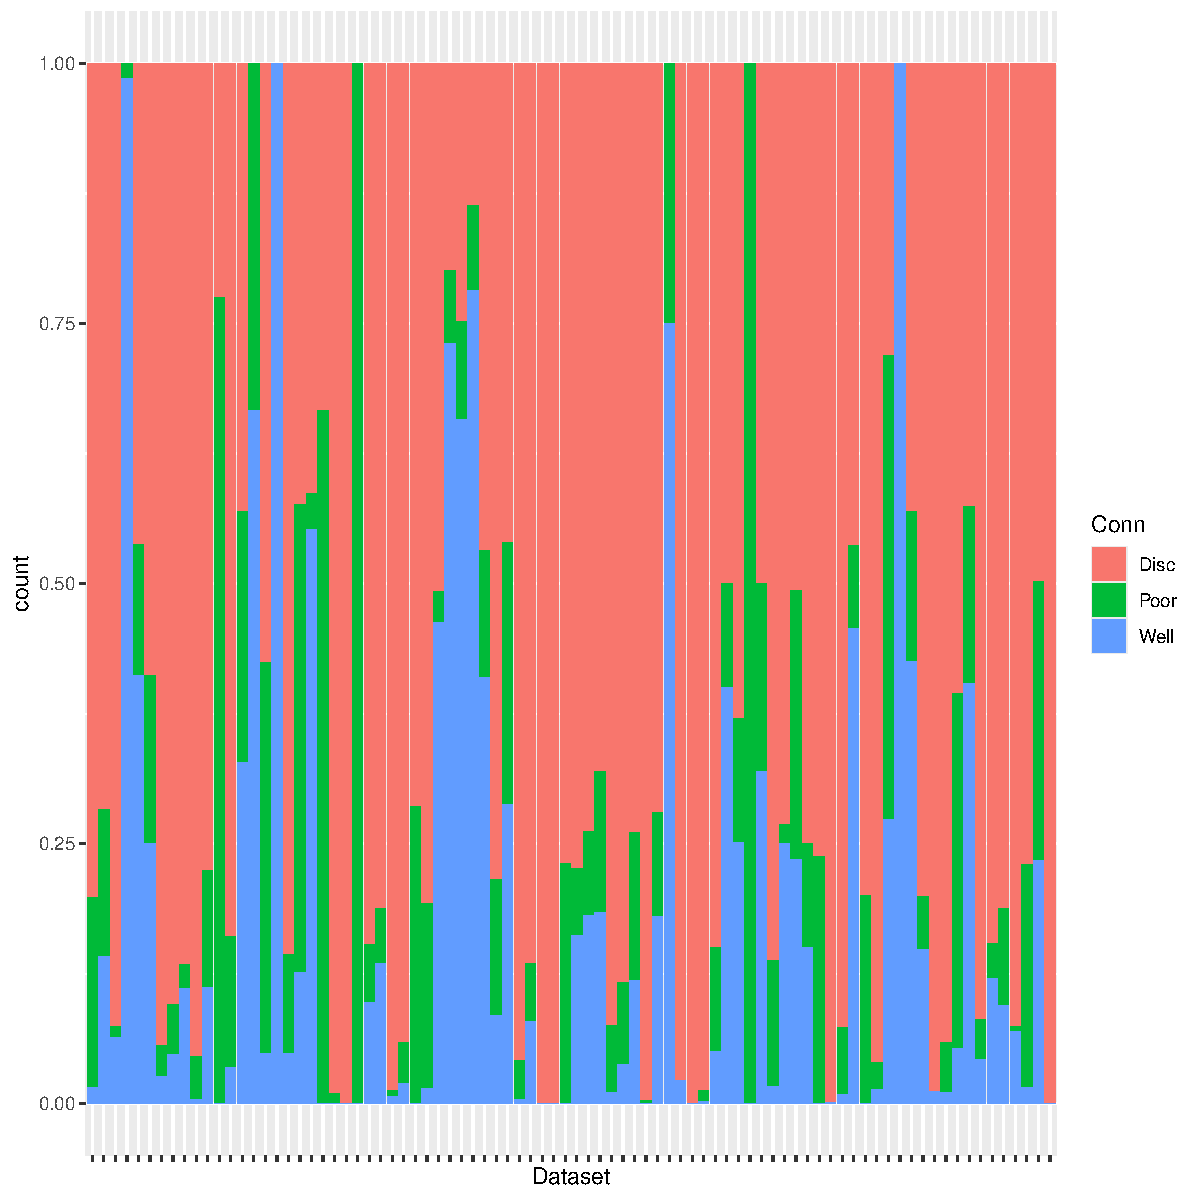
\includegraphics[width=0.4\textwidth]{fig3a.pdf}
	\end{subfloat}
	\begin{subfloat}
		\centering
		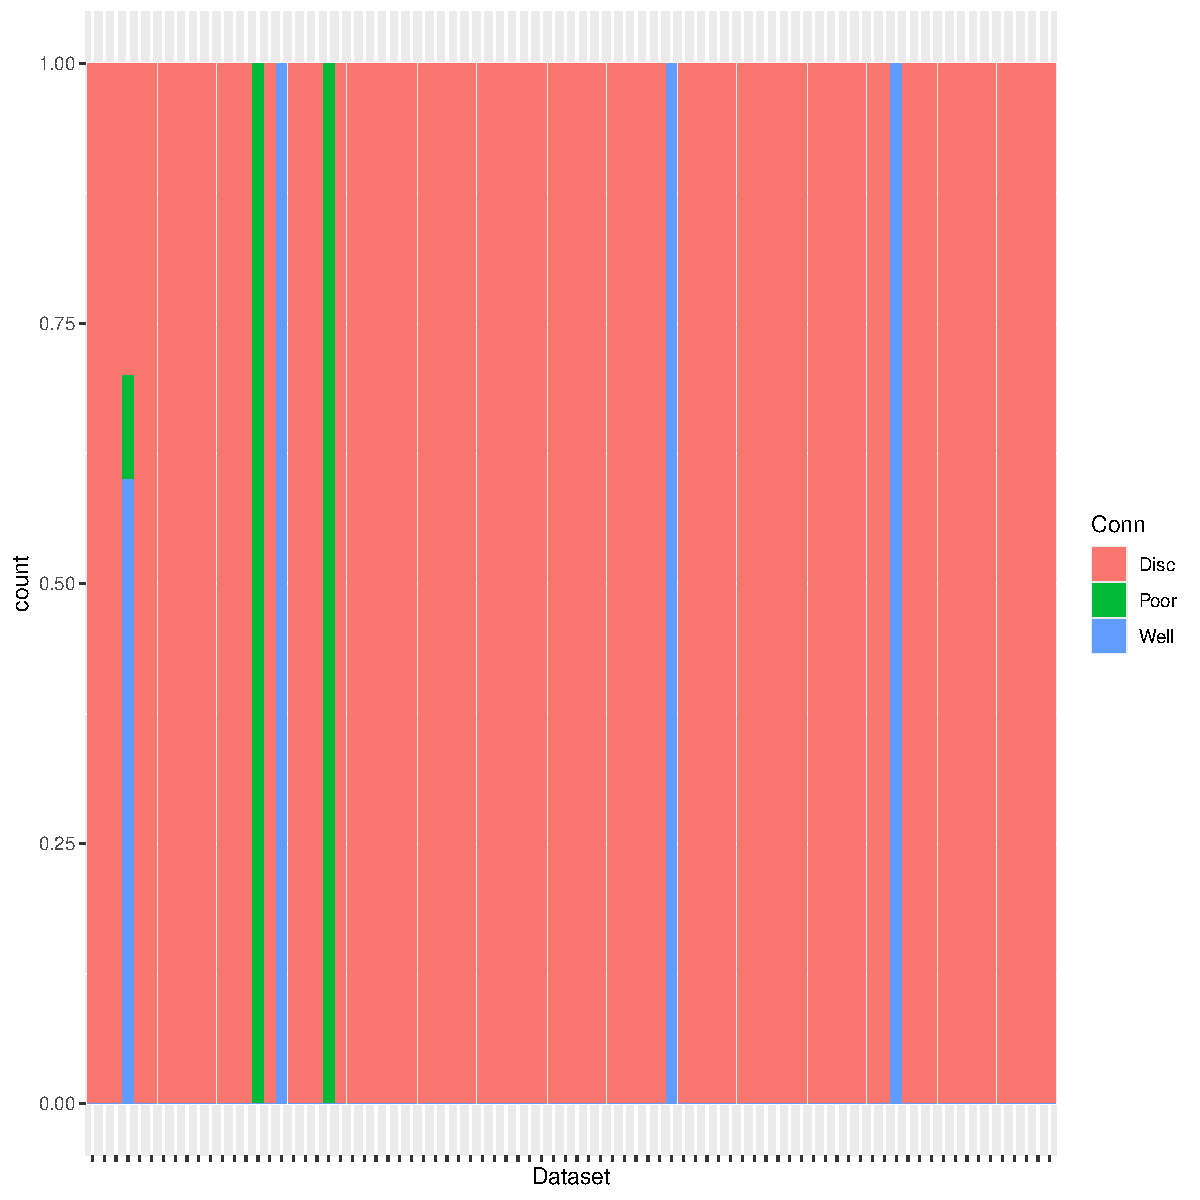
\includegraphics[width=0.4\textwidth]{fig3b.pdf}
	\end{subfloat}
	% \begin{subfloat}
	% 	\centering
	% 	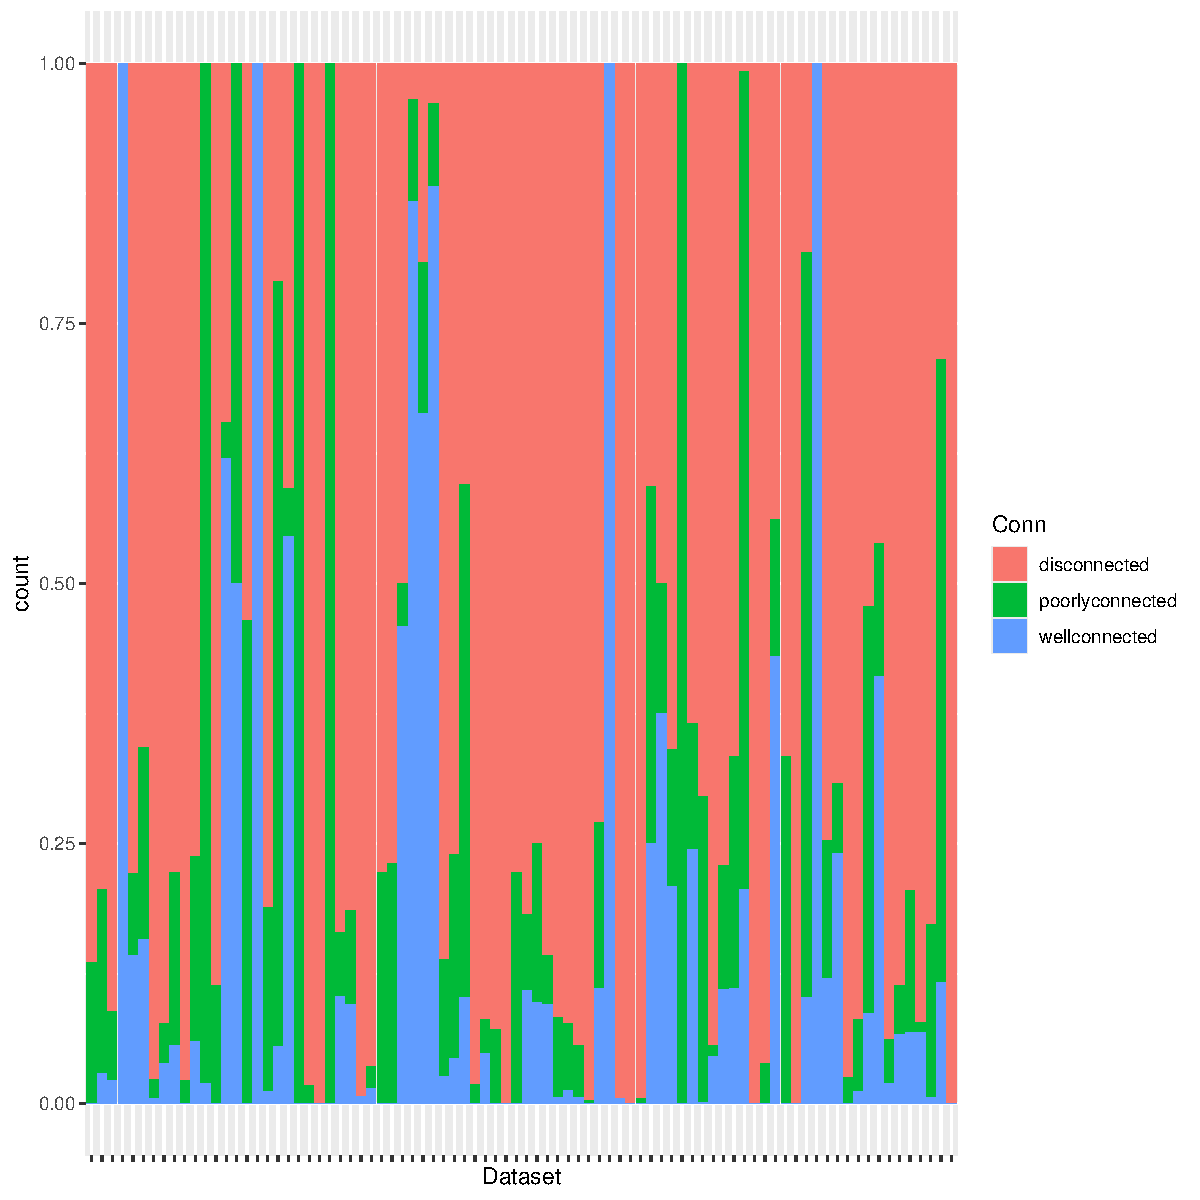
\includegraphics[width=0.8\textwidth]{fig3c.pdf}
	% \end{subfloat}
	\caption{Connectivity of Hierarchical-SBM Clusters.
		On the empirical networks.
		Each bar is a network, sorted in increasing network size.
		The y-axis shows percentage disconnected, poorly-connected $\setminus$ disconnected, and well-connected
		(a) Level0 (b) Level1}
	\label{figs:fig2}
\end{figure}

\begin{figure}[ht]
	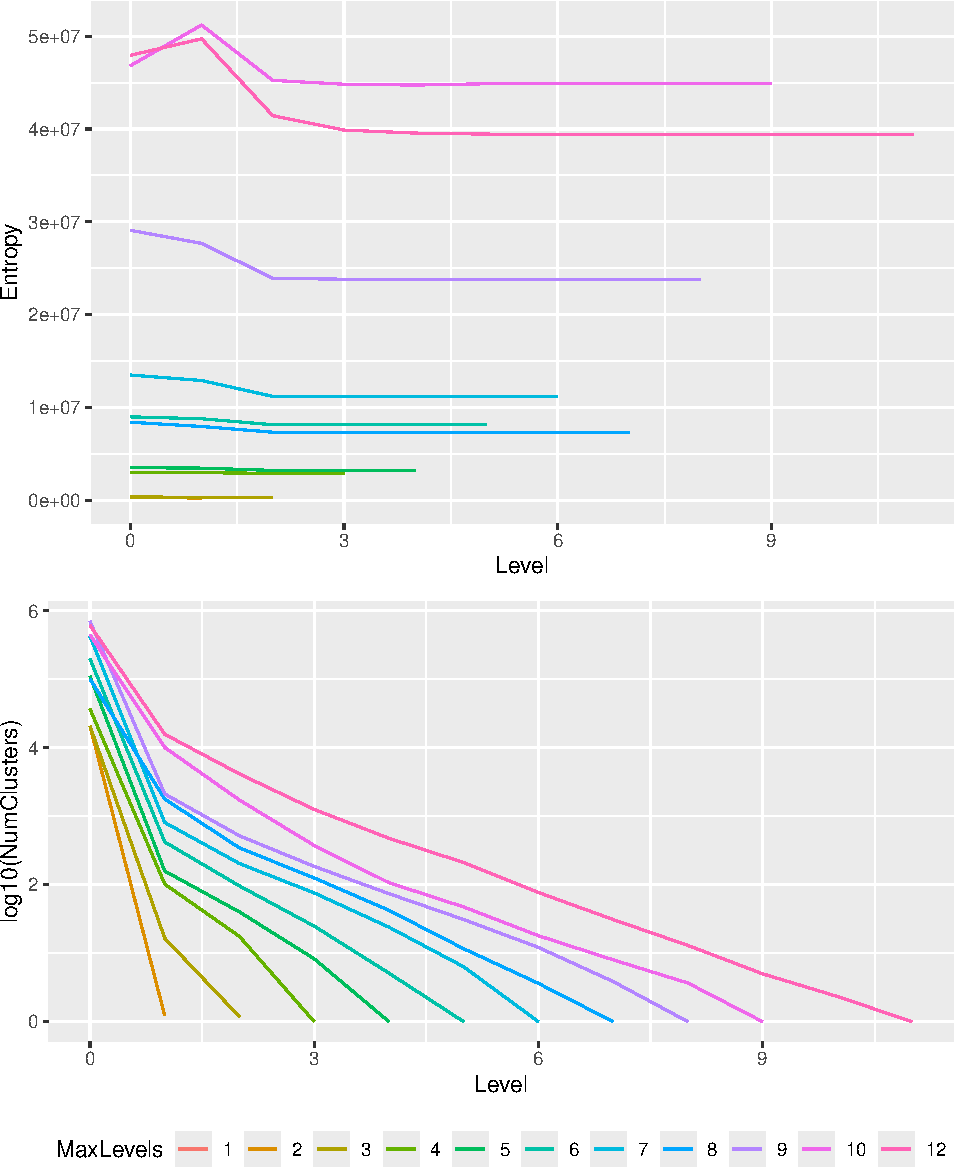
\includegraphics[width=\textwidth]{fig4.pdf}
	\caption{Disconnected Percentage Comparison:
		On the empirical networks.
		We calculate the percentage of disconnected clusters and compare with the non-hierarchical (left) and the hierarchical (right).
	}
	\label{figs:fig3}
\end{figure}

Conducting a paired t-test of disconnected percentages, there is no statistical difference between disconnected percentage (p = 0.5264).
However, comparing the poorly-connected percentage, there is a statistical difference (p = 0.0193).

\clearpage
\bibliography{refs}
\bibliographystyle{ACM-Reference-Format}

\end{document}
